\section{Symulacja i weryfikacja}
\label{sec:sym-wer}

Aby sprawdzić poprawność działania algorytmu optymalizacji dynamicznej, wykonano symulacje weryfikacyjne przy użyciu oprogramowania JModelica.org na wyższym poziomie aplikacji oraz środowiska MATLAB/Simulink na niższym.
W obu tych przypadkach błąd weryfikacji jest liczony według wzoru \ref{eq:ver-error}, gdzie $h_{i}^{s}(T)$ to wartość odpowiedniego poziomu po upływie czasu optymalnego uzyskana w symulacji, a $h_{i}^{f}$ to wartość docelowa tego poziomu.

\begin{equation}\label{eq:ver-error}
e_{wer} = \sum_{i=1}^{3} (h_{i}^{s}(T) - h_{i}^{f})^{2}
\end{equation}

Należy zwrócić uwagę na to, iż weryfikacja poprawności rozwiązania korzysta z innych danych, niż sprawdzenie dokładności rozwiązania opisane w sekcji \ref{sub:opt-dokladnosc}. Pierwsza procedura używa danych symulacyjnych uzyskanych po optymalizacji, a druga - danych pochodzących bezpośrednio z algorytmu optymalizacyjnego.

%-------------------------------------------------
\subsection{Weryfikacja przy użyciu pakietu JModelica.org}
\label{sub:sym-wer-jmodelica}

Po zakończeniu optymalizacji wyższy poziom aplikacji umożliwia przeprowadzenie symulacji weryfikacyjnej. Podaje się wtedy cały uzyskany wektor sterowania optymalnego (w postaci ,,surowej'' lub znormalizowanej) jako trajektorię wejściową do symulacji, a na koniec wylicza się błąd weryfikacji.

Poniżej przedstawiono 2 przykłady wykresów uzyskanych w czasie weryfikacji i porównano wartości błędów przy zastosowaniu sterowania w postaci ,,surowej'' oraz znormalizowanej.

\begin{figure}[htp]
    \centering
    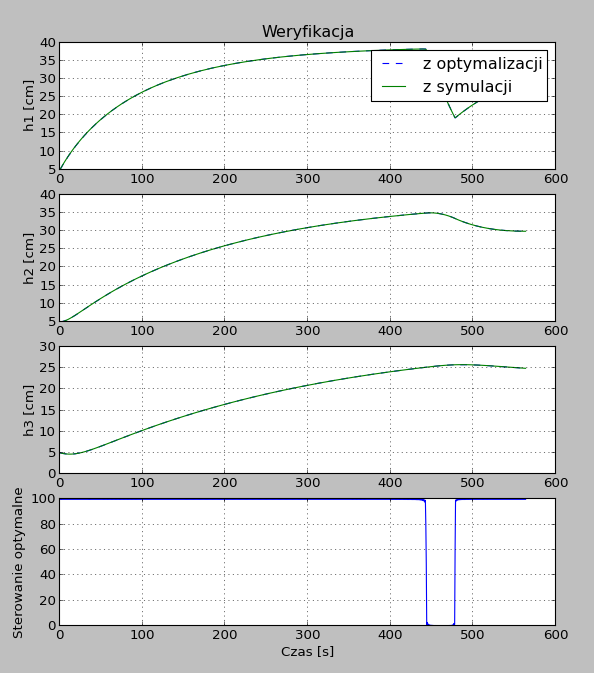
\includegraphics{Grafika/plot_5_5_6-30_30_25-raw-350}
    \caption{Przykładowa weryfikacja rozwiązania przy użyciu pakietu JModelica.org. Źródło: własne.}
    \label{fig:plot556-303035-raw-350}
\end{figure}

\begin{figure}[htp]
    \centering
    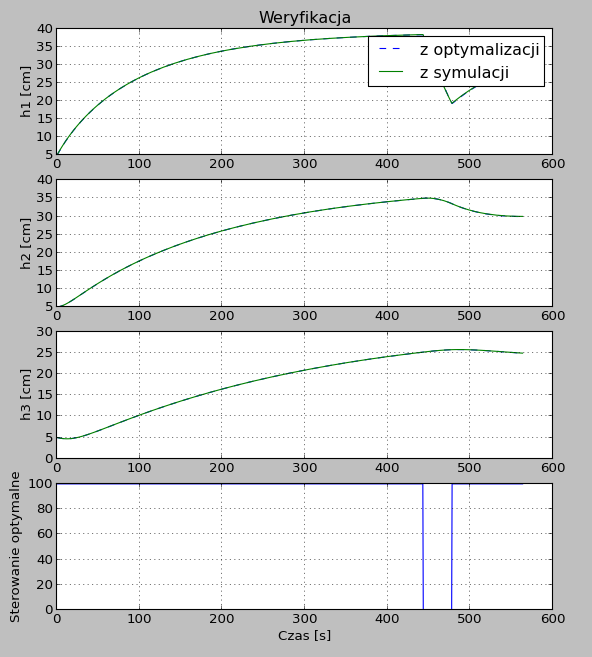
\includegraphics{Grafika/plot_5_5_6-30_30_25-normalised-350}
    \caption{Przykładowa weryfikacja po normalizacji sterowania. Źródło: własne.}
    \label{fig:plot556-303035-normalised-350}
\end{figure}

Pierwszy przykład to napełnianie zbiorników od poziomów $h_{1}^{0} = 5 cm, h_{2}^{0} = 5 cm, h_{3}^{0} = 6 cm$ do poziomów $h_{1}^{f} = 30 cm, h_{2}^{f} = 30 cm, h_{3}^{f} = 25 cm$. Sterowanie w postaci z algorytmu optymalizacji osiągnęło wartość błędu weryfikacji $e_{wer}^{s} = 0,0002$, a po znormalizowaniu: $e_{wer}^{n} = 0.002$. W tym przypadku sterowanie w postaci ,,surowej'' (przedstawione na rys. \ref{fig:plot556-303035-raw-350}) wizualnie nie różni się bardzo od sterowania znormalizowanego (pokazanego na rys. \ref{fig:plot556-303035-normalised-350}), ale nawet taka niewielka różnica może prowadzić do zwiększenia się błędu weryfikacji o rząd wielkości. Jest to jednak również związane z tym, iż pierwszy błąd jest bardzo niewielki i w czasie wielu prób rzadko uzyskiwano tak niewielkie wartości. W tej optymalizacji użyto 350 elementów skończonych.

\begin{figure}[htp]
    \centering
    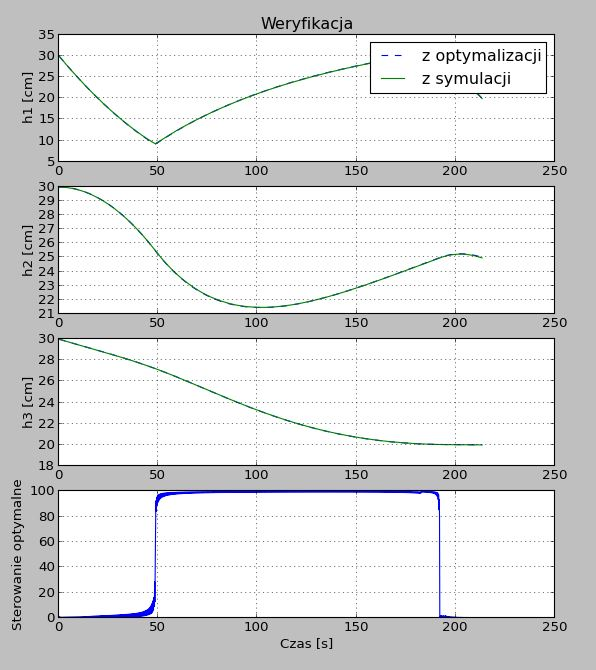
\includegraphics{Grafika/plot_30_30_30-20_25_20_raw_200}
    \caption{Druga przykładowa weryfikacja rozwiązania przy użyciu pakietu JModelica.org. Źródło: własne.}
    \label{fig:plot303030-202520raw200}
\end{figure}

\begin{figure}[htp]
    \centering
    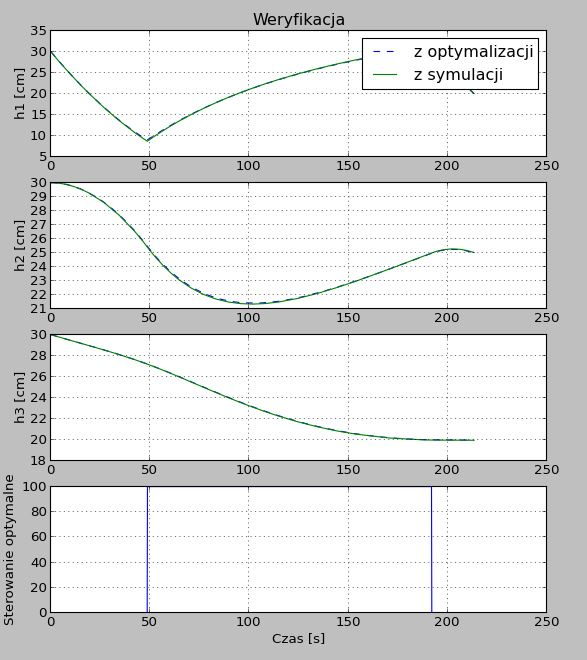
\includegraphics{Grafika/plot_30_30_30-20_25_20_normalised_200}
    \caption{Druga przykładowa weryfikacja po normalizacji sterowania. Źródło: własne.}
    \label{fig:plot303030-202520normalised200}
\end{figure}

Drugi przykład to upuszczanie niewielkiej ilości wody ze zbiorników od poziomów $h_{1}^{0} = 30 cm, h_{2}^{0} = 30 cm, h_{3}^{0} = 30 cm$ do $h_{1}^{f} = 20 cm, h_{2}^{f} = 25 cm, h_{3}^{f} = 20 cm$. Sterowanie w postaci ,,surowej'' osiągnęło wartość błędu weryfikacji $e_{wer}^{s} = 0,007$, a w postaci znormalizowanej: $e_{wer}^{n} = 0.019$. Tutaj różnica między błędami jest mniejsza niż w poprzednim przypadku, mimo bardziej skomplikowanej struktury sterowania wyznaczonego przez algorytm optymalizacyjny (pokazanego na rys. \ref{fig:plot303030-202520raw200}). Sterowanie znormalizowane zaprezentowano na rys. \ref{fig:plot303030-202520normalised200}. W tej optymalizacji użyto 200 elementów skończonych, więc trzeba to wziąć pod uwagę, porównując wartości błędów między oboma opisanymi przypadkami.


\subsubsection{Wpływ liczby elementów metody elementów skończonych na rozwiązanie}

W związku z tym, że zastosowana metoda przynosiła dobre rezultaty, lecz wartości błędu weryfikacji były dosyć duże (rzędu jednej dziesiątej), podjęto próbę zwiększenia liczby elementów skończonych i przeprowadzenia ponownej optymalizacji i weryfikacji. Odkryto, iż istotnie ma ono wpływ na wartość błędów weryfikacji, ale również na czas obliczeń.

Przeprowadzono więc eksperyment, który miał pokazać ten wpływ liczby elementów skończonych na błędy weryfikacji dla sterowania ,,surowego'' i znormalizowanego oraz czas obliczeń. Przyjęto zmianę tej liczby w przedziale 50 do 500 z krokiem 50 tak, aby uzyskać 10 punktów pomiarowych.

W pierwszym przypadku skorzystano z napełniania zbiorników od poziomu $h_{1}^{0} = h_{2}^{0} = h_{3}^{0} = 1 cm$ do $h_{1}^{f} = h_{2}^{f} = h_{3}^{f} = 15 cm$. Uzyskane wyniki przedstawiono na rys. \ref{fig:elementsinfluence1-15_50-500}. Zauważono, iż:
\begin{itemize}
    \item różnica absolutna i relatywna między błędem weryfikacji dla sterowania ,,surowego'' i znormalizowanego jest największa w przypadku najmniejszej rozważanej liczby elementów,
    \item prędkość zmniejszania się błędów
    \item wartości czasów obliczeń rosną najprawdopodobniej wielomianowo,
    \item należy stosować wartości liczby elementów z przedziału między 200 a 350, gdyż tam występuje najlepszy stosunek czasu obliczeń do wartości błędów.
\end{itemize}

\begin{figure}[ht]
    \centering
    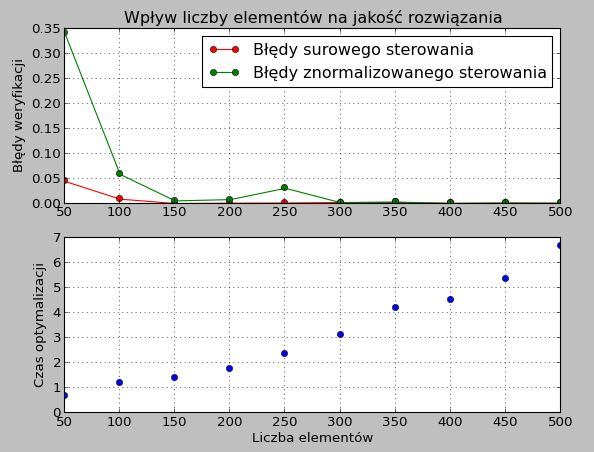
\includegraphics{Grafika/elements_influence_1-15_50-500}
    \caption{Wpływ liczby elementów skończonych na rozwiązanie. Źródło: własne.}
    \label{fig:elementsinfluence1-15_50-500}
\end{figure}

Przeprowadzono drugi eksperyment dla innych danych w celu weryfikacji powyższych wniosków. Tym razem skorzystano z napełniania zbiorników od poziomu $h_{1}^{0} = h_{2}^{0} = h_{3}^{0} = 10 cm$ do $h_{1}^{f} = h_{2}^{f} = h_{3}^{f} = 20 cm$. Wyniki pokazano na rys. \ref{fig:elementsinfluence10-2050-500}. Tym razem zaobserwowano, iż:
\begin{itemize}
    \item wartości błędów są zależne od warunków zadania - w tym przypadku błędy były około 2 razy większe,
    \item czasy obliczeń nie zachowują się tak regularnie, jak w powyższym przypadku i osiągają wartości o rząd wielkości większe, a więc również silnie zależą od warunków zadania,
    \item potwierdziła się hipoteza, iż należy wybierać wartości liczby elementów między 200 a 350.
\end{itemize}

\begin{figure}[ht]
    \centering
    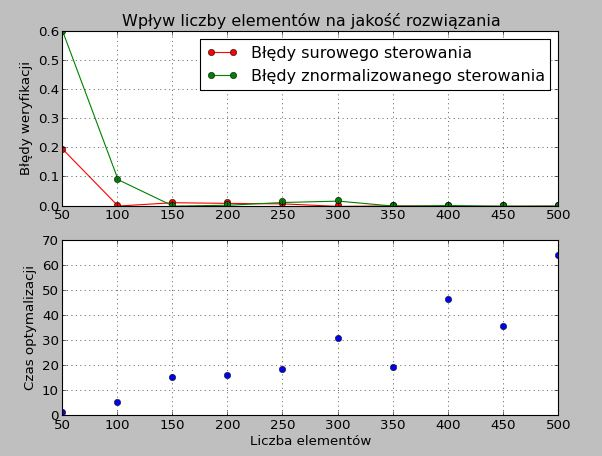
\includegraphics{Grafika/elements_influence_10-20_50-500}
    \caption{Drugi przykład wpływu liczby elementów skończonych na rozwiązanie. Źródło: własne.}
    \label{fig:elementsinfluence10-2050-500}
\end{figure}

\subsubsection{Problemy z błędną wartością pochodnej}

W przypadku niektórych wartości początkowych i końcowych oraz znalezionego dla nich sterowania optymalnego napotykano problem związany z tym, iż pakiet JModelica.org nie był w stanie obliczyć pochodnej jednego ze stanów w punkcie czasu niedługo po pierwszym przełączeniu. Rozwiązano go poprzez zwiększenie liczby elementów skończonych przy rozwiązywaniu danego zadania. Nie zaobserwowano takich problemów przy liczbie elementów powyżej 50.

%-------------------------------------------------
\subsection{Weryfikacja przy użyciu oprogramowania MATLAB/Simulink}
\label{sub:sym-wer-matlab}

%TODO: opisać wykresy i porównać z JModelicą

Symulację weryfikacyjną w programie MATLAB/Simulink przeprowadzono, łącząc oba poziomy aplikacji w całość i uruchamiając odpowiednie obliczenia. Zastosowano tam pewne uproszczenie: symulację uruchamiano dopiero po obliczeniu pierwszego sterowania optymalnego. Pokazano jednak, że w przy kolejnych optymalizacjach dokonywano ich w czasie trwania symulacji i niższy poziom aplikacji był w stanie przełączać się w czasie rzeczywistym między sterowaniem czasooptymalnym a liniowo-kwadratowym.

Poniżej pokazano dwa przykłady funnkcjonowania symulacji weryfikacyjnej niższego poziomu aplikacji.
W obu użyto metody Runge-Kutty 4 rzędu i stałego kroku o wartości 0.001 s. Dobrano taką metodę i wartość kroku czasowego ze względu na przewidywanie możliwości wykorzystania całej opisywanej aplikacji również z rzeczywistym układem zbiorników.
Symulacje przeprowadzono z nieskończonym czasem końcowym, ale prezentowane są tylko interesujące przedziały czasu.

Pierwszy przykład jest pokazany na rys. \ref{fig:extctrl3opts}. Widoczne są tam 3 procesy aplikacji sterowania czasooptymalnego przedzielone okresami, w których działa regulator liniowo-kwadratowy.
Drugi przykład jest przedstawiony na rys. \ref{fig:extctrl2opts} i zawiera 2 procesy aplikacji sterowania czasooptymalnego.
Można je zauważyć na wykresie przedstawiającym sterowanie, gdyż ma ono wtedy postać ,,bang-bang''. W czasie działania regulatora liniowo-kwadratowego sterowanie ma wartość zbliżoną do sterowania ustalonego, które nie leży na ograniczeniach. Nie obserwuje się zbyt dużych zmian sterowania liniowo-kwadratowego, gdyż stan układu jest już w otoczeniu punktu równowagi.

Jak wspominano w podrozdziale \ref{sec:podzial-zadan}, wyznacza się go na podstawie stanu docelowego zagadnienia optymalizacji dynamicznej. Używa się w tym celu metody identycznej z algorytmem inicjalizacyjnym opisanym w sekcji \ref{sub:opt-init}: wyznacza się 3 sterowania ustalone odpowiadające wartościom stanów docelowych w zbiornikach, a następnie wylicza się z nich średnią i traktuje się ją jako sterowanie ustalone dla regulatora liniowo-kwadratowego.

Wyniki weryfikacji porównano z wynikami analogicznych operacji przeprowadzonych przy użyciu wyższego poziomu aplikacji. Podsumowanie wyników zostało przedstawione w tabeli \ref{tab:extctrl3opts} dla pierwszego przykładu i \ref{tab:extctrl2opts} dla drugiego. W jej kolumnach przedstawiono:
\begin{itemize}
    \item czas zakończenia optymalizacji liczony od początku symulacji,
    \item stan początkowy układu użyty do wyznaczenia sterowania czasooptymalnego,
    \item stan docelowy układu,
    \item błąd weryfikacji obliczony na niższym poziomie aplikacji w programie MATLAB/Simulink,
    \item błąd weryfikacji obliczony na wyższym poziomie aplikacji przy użyciu platformy JModelica.org; obliczono go, używając 350 elementów skończonych w algorytmie optymalizacji i normalizując sterowanie.
\end{itemize}

\begin{figure}
    \centering
    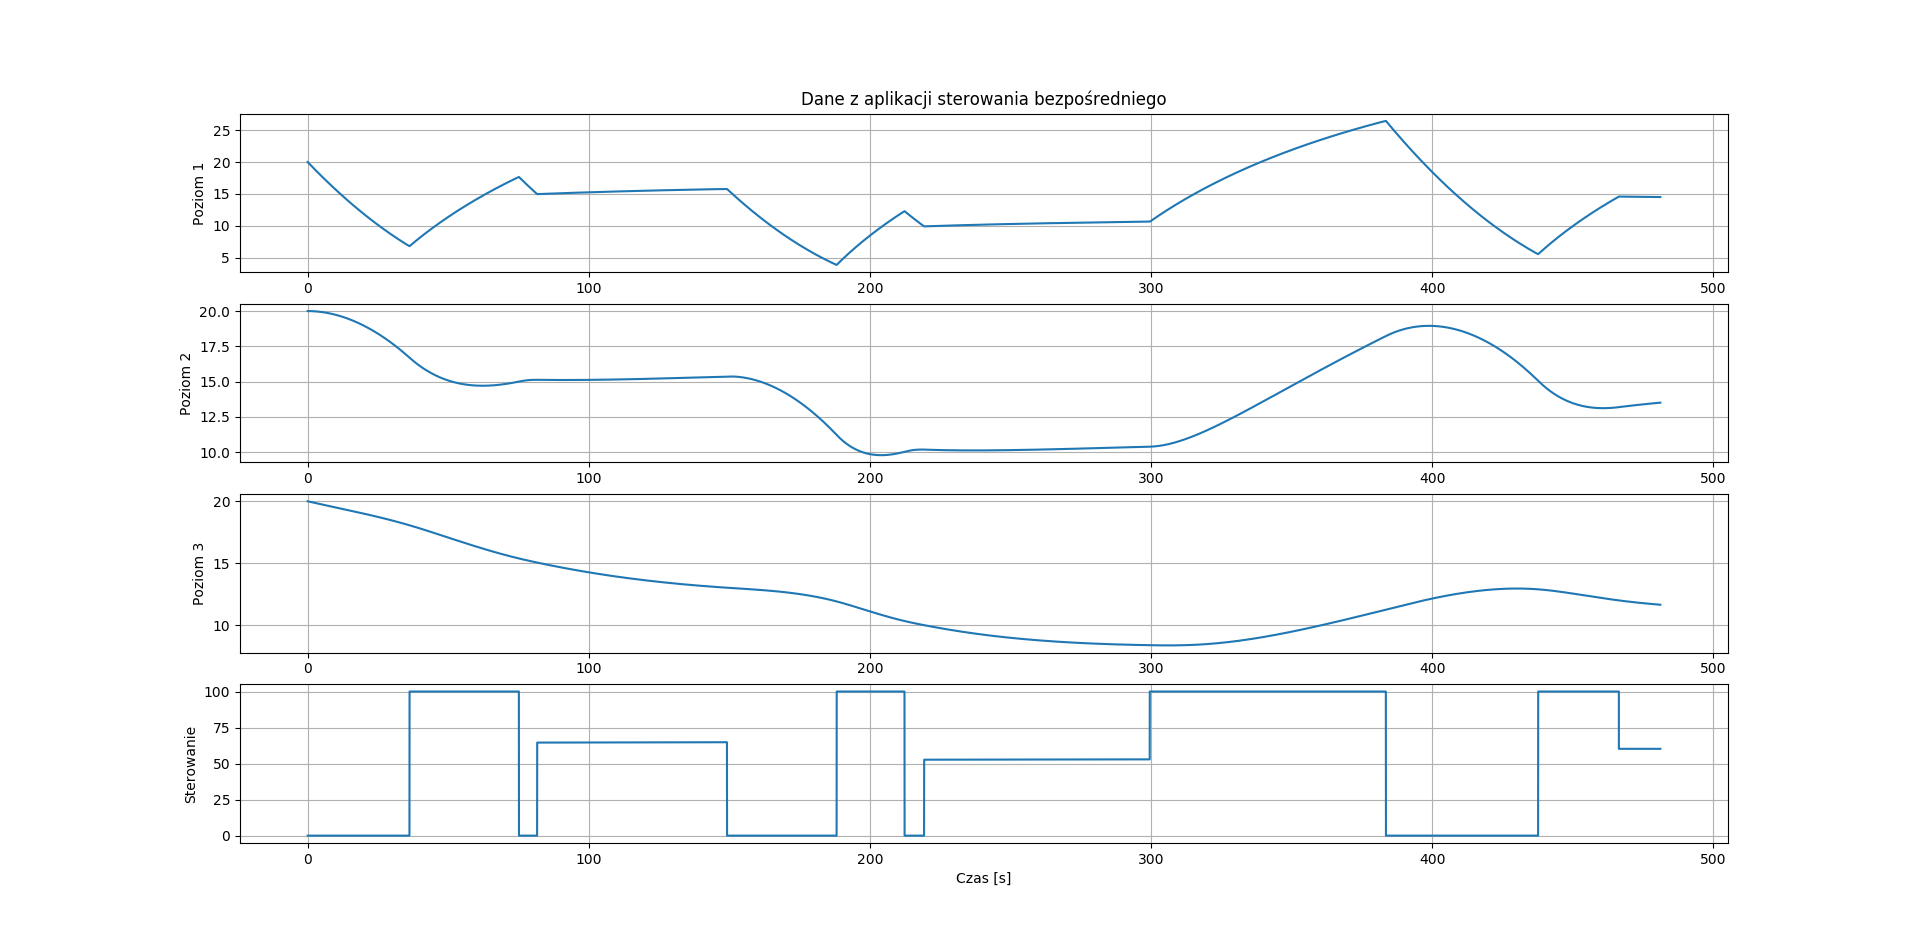
\includegraphics[scale=0.5,angle=90]{Grafika/ext_ctrl_3_opts}
    \caption{Trzy procesy optymalizacji zweryfikowane w symulacji niższego poziomu aplikacji. Źródło: własne.}
    \label{fig:extctrl3opts}
\end{figure}


\begin{table}[htp]
    \centering
    \begin{tabular}{|c|c|c|c|c|}
        \hline 
        \textbf{Czas} & \textbf{Stan początkowy} & \textbf{Stan docelowy} & \textbf{$e_{MATLAB}$} & \textbf{$e_{JModelica.org}$} \\ 
        \hline 
        81,623 & $h^{0} = [20 ~20~ 20]^{T}$ & $h^{f} = [15 ~15~ 15]^{T}$ & 0,021 & 0,008 \\ 
        \hline 
        219,268 & $h^{0} = [15.77~ 15.37~ 13.02]^{T}$ & $h^{f} = [10 ~10~ 10]^{T}$ & 0,047 & 0,0095 \\ 
        \hline 
        466,422 & $h^{0} = [10.62~ 10.39~ 8.37]^{T}$ & $h^{f} = [15 ~13~ 12]^{T}$ & 0,221 & 0,0007 \\ 
        \hline 
    \end{tabular}
\caption{Podsumowanie wyników weryfikacji wyższego i niższego poziomu aplikacji dla trzech optymalizacji przedstawionych na rys. \ref{fig:extctrl3opts}. Źródło: własne.}
\label{tab:extctrl3opts}
\end{table}

\begin{figure}
    \centering
    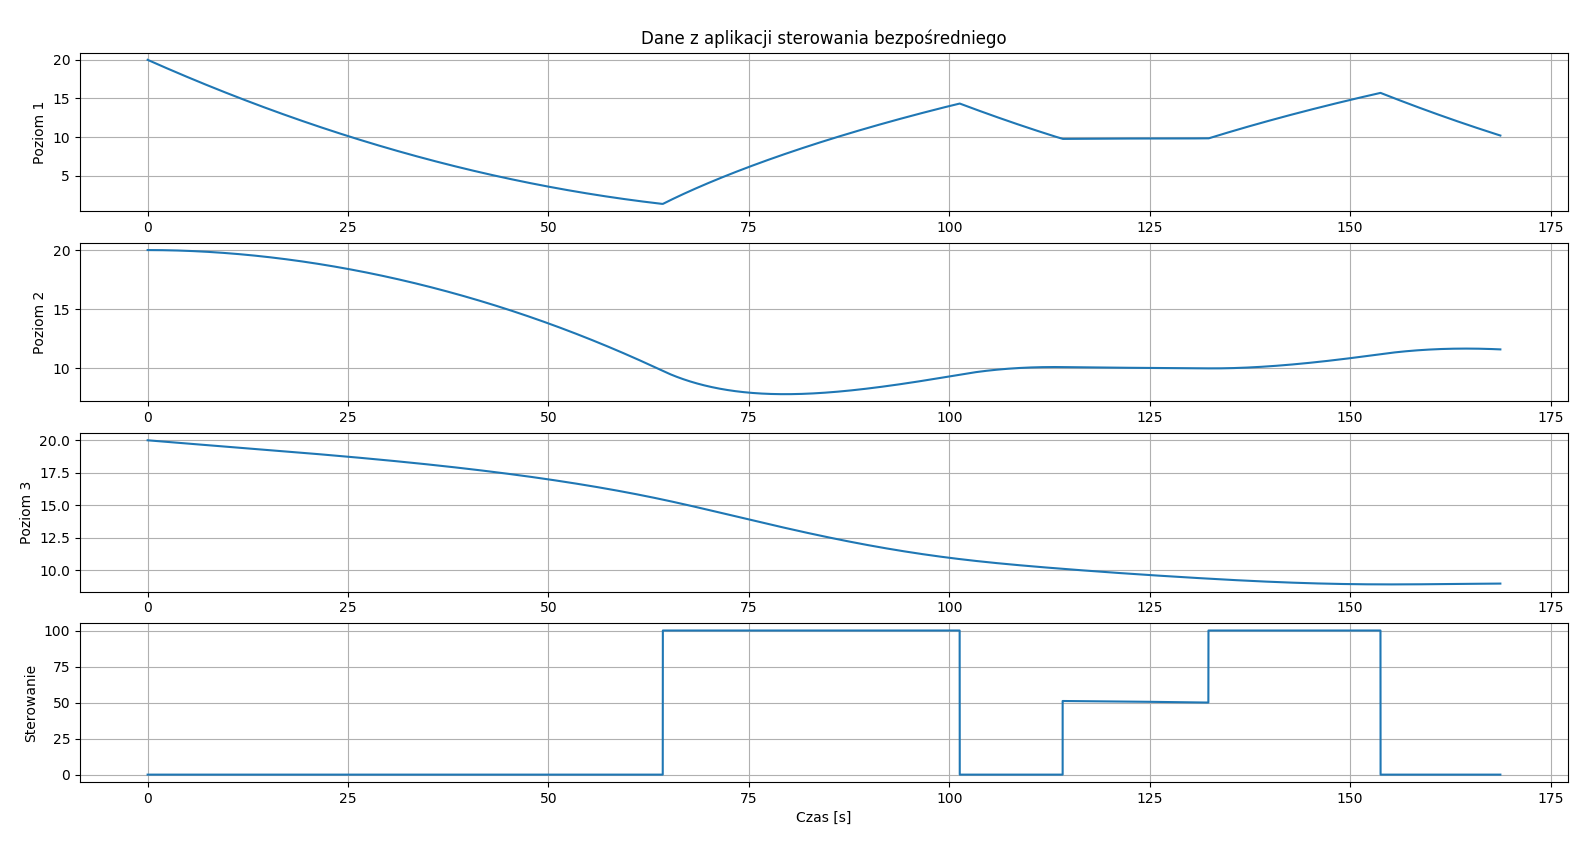
\includegraphics[scale=0.5,angle=90]{Grafika/ext_ctrl_2_opts}
    \caption{Dwa procesy optymalizacji zweryfikowane w symulacji niższym poziomem aplikacji. Źródło: własne.}
    \label{fig:extctrl2opts}
\end{figure}

\begin{table}[htp]
    \centering
    \begin{tabular}{|c|c|c|c|c|}
        \hline 
        \textbf{Czas} & \textbf{Stan początkowy} & \textbf{Stan docelowy} & \textbf{$e_{MATLAB}$} & \textbf{$e_{JModelica.org}$} \\
        \hline 
        114,141 & $h^{0} = [20~ 20~ 20]$ & $h^{f} = [10 ~10~ 10]^{T}$ & 0,081 & 0,002 \\ 
        \hline 
        168,743 & $h^{0} = [9.82~ 9.99~ 9.37]$ & $h^{f} = [10 ~12~ 9]^{T}$ & 0,203 & 0,0005 \\ 
        \hline 
    \end{tabular}
    \caption{Podsumowanie wyników weryfikacji wyższego i niższego poziomu aplikacji dla dwóch optymalizacji przedstawionych na rys. \ref{fig:extctrl2opts}. Źródło: własne.}
    \label{tab:extctrl2opts}
\end{table}

Zauważono, iż błędy weryfikacji na niższym poziomie rosną przy kolejnych optymalizacjach. Dzieje się tak ze względu na fakt, iż aplikacja wyższego poziomu przeprowadza optymalizację na podstawie danych pobranych przed uruchomieniem algorytmu, ale sterowanie jest wysyłane na niższy poziom po zakończeniu jej działania. Przez czas działania algorytmu poziomy zmieniają się jednak i dążą dalej do odpowiedniego punktu równowagi. Ten problem mógłby rozwiązać układ predykcyjny działający po stronie wyższego poziomu aplikacji, który wyznaczałby spodziewane wartości poziomów początkowych w momencie rozpoczęcia aplikacji sterowania czasooptymalnego. Jednakże jak pokazano w sekcji \ref{sub:sym-wer-jmodelica}, czas działania algorytmu optymalizacji jest różny dla różnych zestawów stanów początkowych i końcowych, a jego oszacowanie mogłoby być trudnym zadaniem.

Błędy pierwszych optymalizacji nie powinny być obarczone tym problemem, ale i tak są o rząd wielkości większe od tych uzyskanych na wyższym poziomie aplikacji. Jest to najprawdopodobniej spowodowane niedokładnością wyznaczenia czasów przełączeń: w aplikacji wyższego poziomu do weryfikacji podaje się cały wektor sterowania, a w aplikacji niższego poziomu używa się tylko czasów przełączeń, które mogą być obarczone numerycznym błędem obcięcia.
